\newpage
\section{Optymalizacja \label{sec:optim}}
\subsection{Kontekst historyczny \label{subsec:hist}}
    Poszukiwanie ...
\subsection{Specyfikacja zadania optymalizacji \label{subsec:specOptim}}

Ze względu na zróżnicowanie dziedzin, w których możliwe jest sformułowanie 
problemu optymalizacji, wygodnie jest przedstawić specyfikację tego problemu na wysokim poziomie abstrakcji. W ogólności zadanie optymalizacji można przedstawić w postaci następującej krotki: 

\begin{equation}
   Opt =  <\mathcal{I}, \mathcal{O}, \preceq_{O}, f, c>
\end{equation}

w której $\mathcal{I}$ jest dziedziną wejściową problemu, \mathcal{O} dziedziną wyjściową lub zbiorem rozwiązań, na którym określona jest relacja częściowego porządku $\preceq_{O}$. Obie struktury w toku dalszych rozważań należy utożsamiać ze zbiorami. Morfizm 
\begin{equation*}
    f\colon\; \mathcal{I} \rightarrow \mathcal{O}
\end{equation*}
przekształca elementy dziedziny $\mathcal{I}$ w elementy zbioru rozwiązań $\mathcal{O}$, na których określony jest predykat 

\begin{equation*}
    c\colon\; \mathcal{O} \rightarrow \{0, 1\}
\end{equation*}
sprawdzający dopuszczalność rozwiązania. Celem zadania optymalizacyjnego jest znalezienie takiej instancji dziedziny $ \hat{i} \in \mathcal{I}$, dla której zachodzi następująca relacja:

\begin{equation}
    \label{opt-pred}
    \forall{ i \in \mathcal{I} && i \neq \hat{i}} f\left(\hat{i}\right) \preceq_{\mathcal{O}} f\left(i\right).
\end{equation}

Przy czym element $\hat{i}$ nazywany jest \textbf{optimum globalnym}. W praktycznych problemach optymalizacyjnych znalezienie optimum globalnego jest często bardzo trudne lub w przypadku problemów NP-trudnych -- niemożliwe w akceptowalnym czasie. Z tego względu poszukiwane jest \textbf{optimum lokalne} $\bar{i}$, dla którego zachodzi (\ref{opt-pred}), ale tylko w pewnym podzbiorze $\mathcal{I}$. Graficzna reprezentacja problemu optymalizacji znajduje się na \ref{fig:optim-spec}.
\begin{figure}
    \centering
    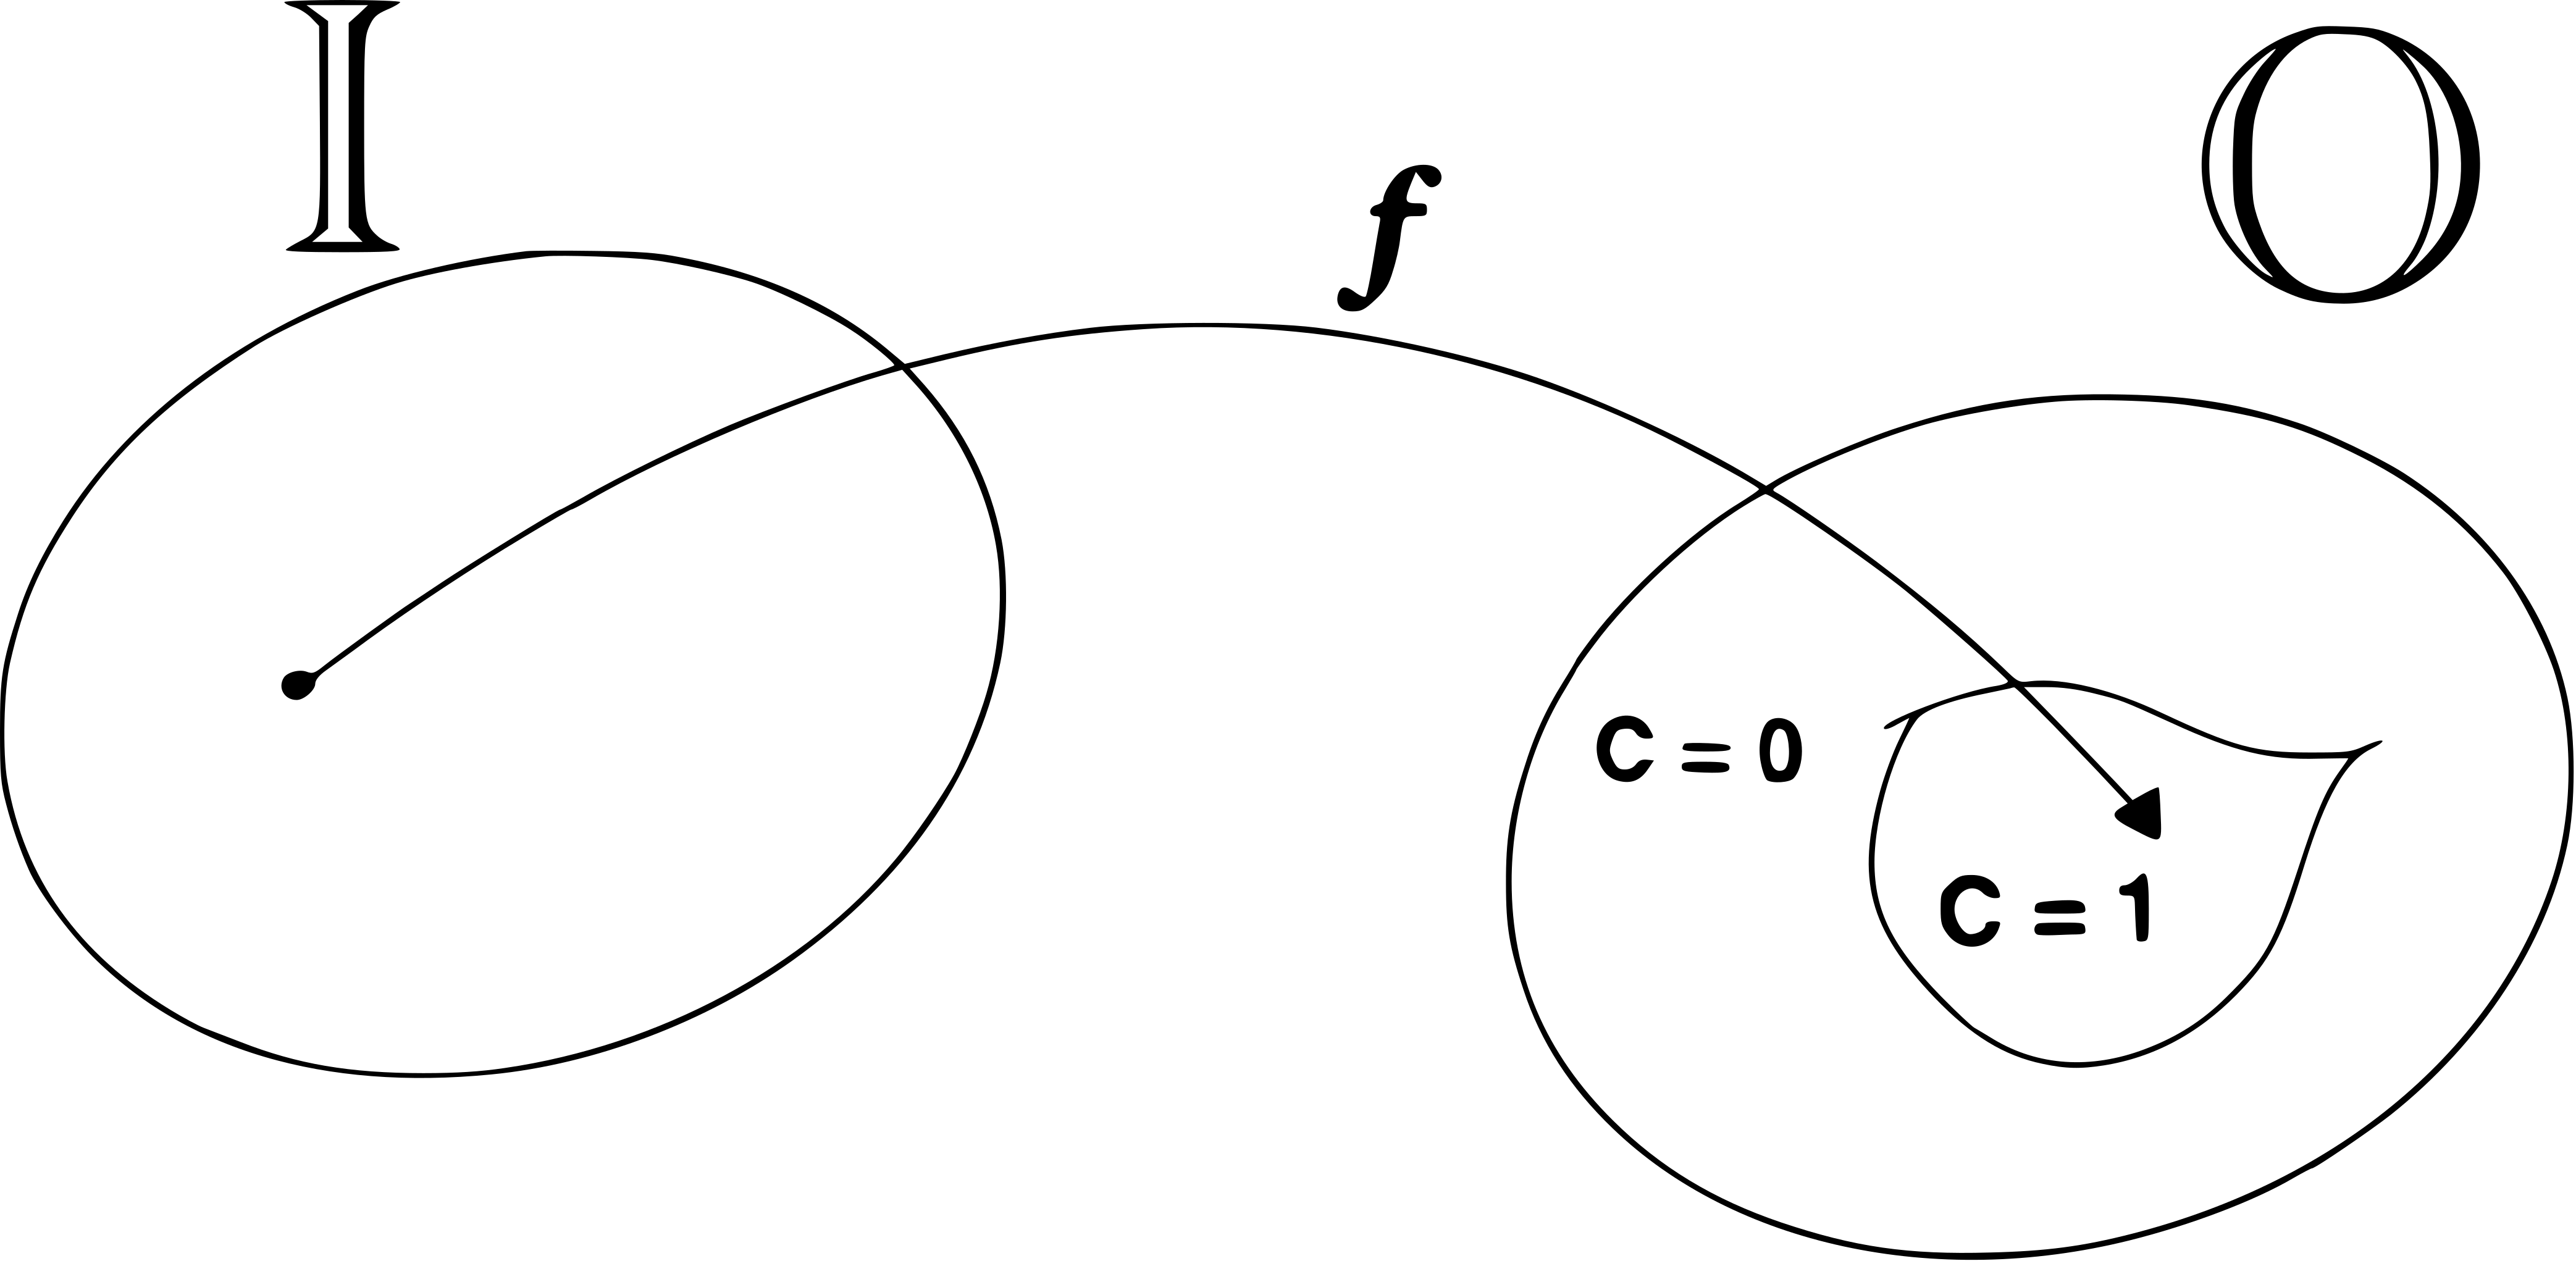
\includegraphics[width=0.65\textwidth]{thesis/img/png-file.png}
    \caption{Geometryczna reprezentacja problemu optymalizacyjnego.}
    \label{fig:optim-spec}
\end{figure}
Ponadto w powyższej specyfikacji zadanie optymalizacyjne utożsamione zostało z zadaniem minimalizacji. Przekształcenie zadania minimalizacji w zadanie optymalizacji lub odwrotnie jest trywialne i sprowadza się do zamiany miejscami operandów relacji $\preceq_{\mathcal{O}}$. W dalszej części pracy zadanie optymalizacji będzie rozumiane wyłącznie jako zadanie minimalizacji.


\subsection{Taksonomia problemów optymalizacyjnych \label{subsec:takson}}

Wyprowadzony model zadania optymalizacyjnego w podrozdziale \ref{subsec:specOptim} pozwala 
myśleć o tym zadaniu jako o abstrakcyjnie typie danych, w którym specyfikacja konkretnych składowych, wyznacza rodzaj zadania optymalizacyjnego. W niniejszym rozdziale zostaną przedstawione i pokrótce opisane najczęściej spotykane typy zadań optymalizacyjnych. \\

\paragraph{Podział ze względu na dziedzinę wejściową}

W przypadku dziedziny wejściowej $\mathcal{I}$ mówi się o optymalizacji ciągłej, jeśli zbiór ten jest nieprzeliczalny, lub o optymalizacji dyskretnej, jeśli zbiór jest przeliczalny. Ponadto w klasie problemów dyskretnych wprowadza się podział na problemy programowania całkowitoliczbowego (ang. \textit{integer programming}), w których elementy dziedziny wejściowej są tożsame wektorom liczb całkowitych, tj.:
\begin{equation*}
    \mathcal{I} = \mathbb{Z}^{n},\; n \geq 1.
\end{equation*}

\paragraph{Podział ze względu na zbiór rozwiązań}

\paragraph{Podział ze względu na funkcję celu}

\paragraph{Podział ze względu na ograniczenia}

\subsection{Algorytm optymalizacyjny \label{subsec:optim-alg}}

\subsection{Taksonomia algorytmów optymalizacyjnych \label{subsec:optim-alg-takson}}
